\chapter{Experiences}
\label{sec:experiences}

\section{Samples}

Sample characterization


\section{Uncovering important variables}


\subsection{Feature importance and correlation with RandomForestClassifier}

The following experiments were designed using the RandomForestClassifier algorithm \cite{scikit-learn}. The goal was to obtain important features that would be able to explain the occurrence of wildfires. These tests were conducted on the three samples previously mentioned.

Firstly, for each sample, a wildfire occurrence was set 3 hours before the wildfire occurrence and 1 hour after, and then the most important variables were calculated. Their complete hourly records were used. With a random state of 445621151 for RandomForestClassifier, the tables \ref{importance_2015_2019} and \ref{importance_2022} show the results for each year.

\begin{table}[H]
	\caption{Variable importance for 2015 and 2019}
	\label{importance_2015_2019}
	\centering
	\begin{tabular}{llll}
		\multicolumn{1}{|l}{2015}      & \multicolumn{1}{l|}{} & 2019                              & \multicolumn{1}{l|}{} \\ \hline
		Variable                       & Importance            & Variable                          & Importance            \\
		soil\_moisture\_100\_to\_255cm & 0.122                 & wind\_speed\_100m                 & 0.072                 \\
		DMC                            & 0.057                 & soil\_temperature\_100\_to\_255cm & 0.065                 \\
		ISI                            & 0.053                 & BUI                               & 0.062                 \\
		BUI                            & 0.051                 & soil\_temperature\_7\_to\_28cm    & 0.056                 \\
		wind\_speed\_100m              & 0.042                 & soil\_moisture\_100\_to\_255cm    & 0.053                
	\end{tabular}
\end{table}

\begin{table}[H]
	\caption{Variable importance for 2022}
	\label{importance_2022}
	\centering
	\begin{tabular}{ll}
		\hline
		2022     &            \\ \hline
		Variable & Importance \\
		DMC      & 0.127      \\
		BUI      & 0.111      \\
		DC       & 0.087      \\
		ISI      & 0.054      \\
		FWI      & 0.052     
	\end{tabular}
\end{table}

For the following experiments, the three samples were concatenated into one. The last 24 rows of each sample were assigned as 1 in the boolean scale of wildfire occurrence, while the rest were assigned as 0. With the RandomForestClassifier algorithm, it was possible to obtain the data shown in Table \ref{hourly_values} depicting the five most important features according to this method.
The two least important features are \textit{rain} and \textit{precipitation}. Although \textit{rain} was considered one of the least important features, it cannot be discarded because it is a variable in \textit{FWI} component analysis, and three components from \textit{FWI} are among the most important features that appear in table \ref{hourly_values}.
In relation to wildfire correlation, wind and soil moisture are the most prevalent variables present with a negative correlation in table \ref{hourly_values_correlation}. Different depths of soil moisture appear in the positive and negative spectrum of correlation.

\begin{table}[H]
	\caption{Variable importance for hourly values}
	\centering
	\label{hourly_values}
	\begin{tabular}{lc}
		\hline
		Variable                       & \multicolumn{1}{l}{Importance} \\ \hline
		soil\_moisture\_100\_to\_255cm                             & 0.096                          \\
		soil\_moisture\_7\_to\_28cm                            & 0.081                          \\
		DMC & 0.081                          \\
		DC                            & 0.077                          \\
		BUI              & 0.070                       
	\end{tabular}
\end{table}

\begin{table}[H]
	\caption{Variable correlation to wildfire}
	\centering
	\label{hourly_values_correlation}
	\begin{tabular}{lc}
		\hline
		Variable                       & \multicolumn{1}{l}{correlation} \\ \hline
		surface\_pressure                             & 0.105                          \\
		soil\_temperature\_100\_to\_255cm                            & 0.060                          \\
		soil\_moisture\_0\_to\_7cm & 0.0602                          \\
		dew\_point\_2m                            & 0.026                          \\
		soil\_moisture\_7\_to\_28cm              & 0.023   \\
		soil\_moisture\_100\_to\_255cm & -0.155 \\
		soil\_moisture\_28\_to\_100cm & -0.131 \\
		wind\_speed\_100m & -0.097 \\
		wind\_speed\_10m & -0.095 \\
		wind\_gusts\_10m & -0.080 \\                   
	\end{tabular}
\end{table}



Table \ref{daily_values} displays the five most important features, according to a daily average value. For each variable, a mean value was calculated, and it was assigned to the last day as a boolean value for wildfire 1, depicting an occurrence of a wildfire. This method showed little difference in relation to the values shown in table \ref{hourly_values}. The two least important features considered were \textit{precipitation} and \textit{dew\_point\_2m}. Both table \ref{hourly_values_correlation} and table \ref{daily_values_correlation} do not show the most common variables associated with wildfires (temperature and humidity) as the ones with the most correlation to a wildfire occurrence. 
\begin{table}[H]
	\caption{Variable importance with daily mean method}
	\centering
	\label{daily_values}
	\begin{tabular}{lc}
		\hline
		Variable                        & \multicolumn{1}{l}{Importance} \\ \hline
		wind\_speed\_100m  & 0.115                          \\
		soil\_moisture\_100\_to\_255cm   & 0.093                          \\
		wind\_speed\_10m          & 0.066                          \\
		terrestrial\_radiation\_instant               & 0.058                          \\
		soil\_moisture\_7\_to\_28cm & 0.056                         
	\end{tabular}
\end{table}


\begin{table}[H]
	\caption{Variable correlation to wildfire daily mean}
	\centering
	\label{daily_values_correlation}
	\begin{tabular}{lc}
		\hline
		Variable                       & \multicolumn{1}{l}{correlation} \\ \hline
		surface\_pressure                             & 0.110                         \\
		soil\_moisture\_0\_to\_7cm                            & 0.061                          \\
		soil\_temperature\_100\_to\_255cm & 0.060                          \\
		dew\_point\_2m                            & 0.035                          \\
		cloud\_cover\_mid              & 0.028   \\
		soil\_moisture\_100\_to\_255cm & -0.155 \\
		wind\_speed\_10m & -0.151 \\
		wind\_speed\_100m & -0.149 \\
		soil\_moisture\_28\_to\_100cm & -0.131 \\
		wind\_gusts\_10m & -0.122 \\                   
	\end{tabular}
\end{table}


Another experiment was conducted by selecting a time frame between 9:00 and 20:00 hours. Taking a glace at figure \ref{fig:daily_fwix_2015_2019_2020}, the value of \textit{FWI} starts to increase around 8 or 9 in the morning, has its highest value around 15, and then it starts to decrease. After around 20 hours, it reaches its lowest point in the samples from the years 2015 and 2019. 


Table \ref{hourly_importance_fwix_2015_2019_2020} shows soil moisture as the most important feature, like in Table \ref{hourly_values}. There was also another experiment where the time frame was selected according to the hour of the wildfire. 


\begin{figure}[h]
	\centering
	\caption{Hourly FWI value for the day of wildfire occurence}
	\begin{subfigure}{0.45\textwidth}
		\centering
		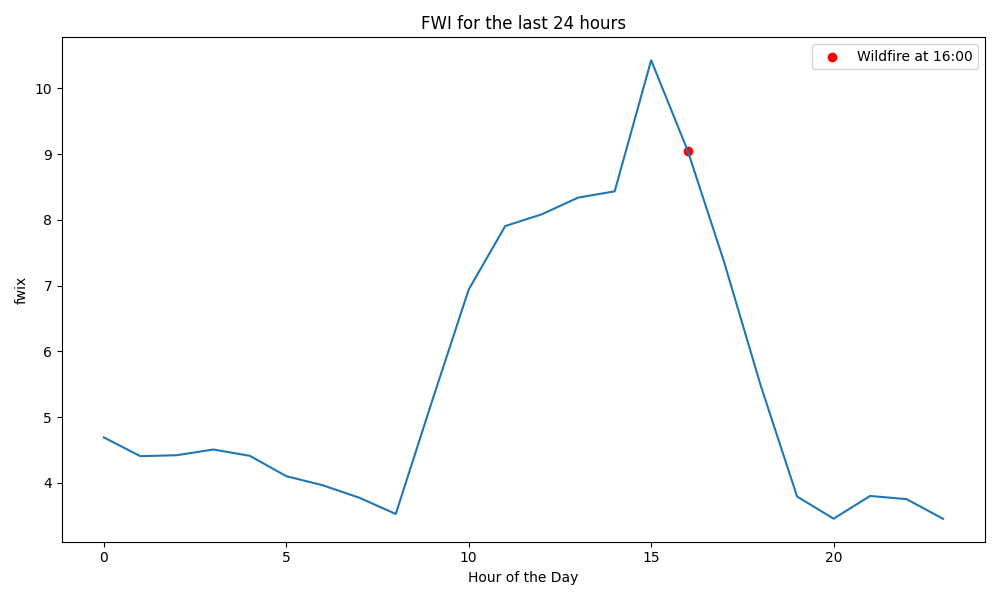
\includegraphics[width=\textwidth]{graphs/variables/fwix_24_2015.png}
		\caption{2015}
	\end{subfigure}
	\hfill
	\begin{subfigure}{0.45\textwidth}
		\centering
		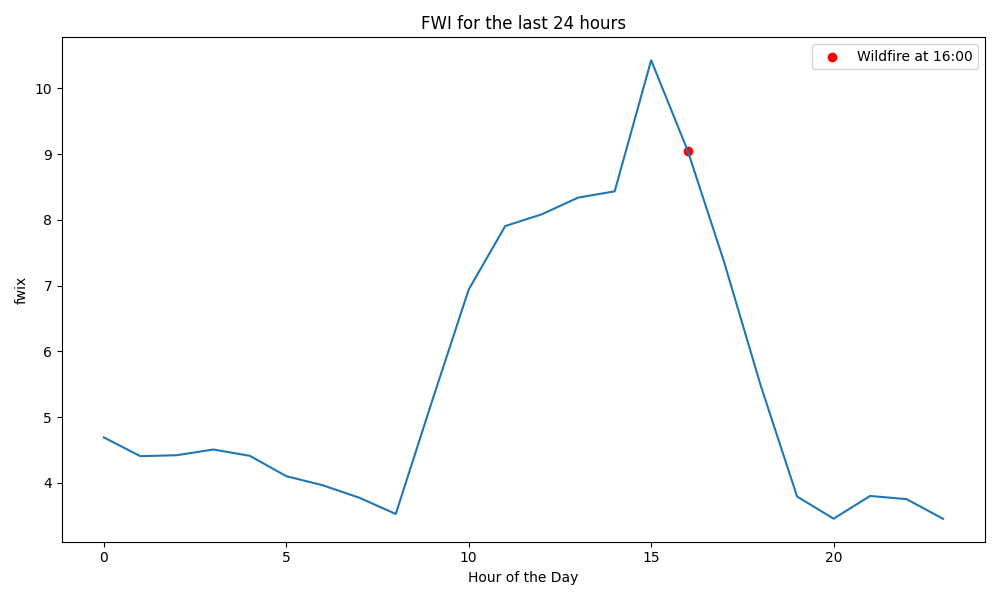
\includegraphics[width=\textwidth]{graphs/variables/fwix_24_2015.png}
		\caption{2019}
	\end{subfigure}
	\hfill
	\begin{subfigure}{0.45\textwidth}
		\centering
		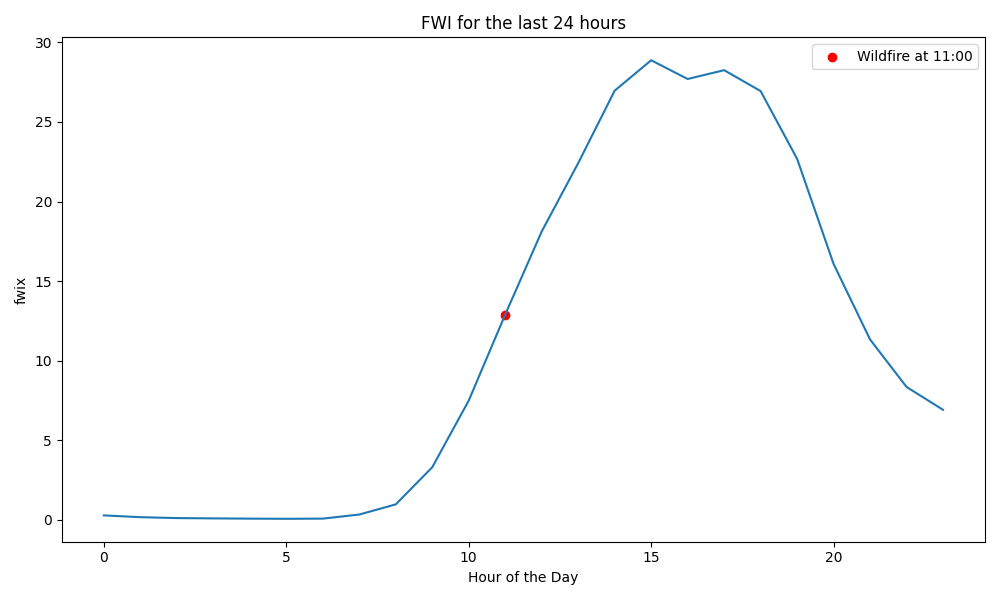
\includegraphics[width=\textwidth]{graphs/variables/fwix_24_2019.png}
		\caption{2022}
	\end{subfigure}
	
	\label{fig:daily_fwix_2015_2019_2020}
\end{figure}

\begin{table}[H]
	\centering
	\caption{Variable importance with \textit{FWI} time frame method}
	\begin{tabular}{lc}
		\hline
		Variable                       & \multicolumn{1}{l}{Importance} \\ \hline
		soil\_moisture\_100\_to\_255cm & 0.073                          \\
		DMC                            & 0.072                          \\
		soil\_moisture\_7\_to\_28cm                             & 0.072                          \\
		DC    & 0.057                          \\
		soil\_moisture\_28\_to\_100cm                            & 0.049                         
	\end{tabular}
	\label{hourly_importance_fwix_2015_2019_2020}
\end{table}

\begin{table}[H]
	\caption{Variable correlation to wildfire time frame method}
	\centering
	\label{hourly_correlation_fwix_2015_2019_2020}
	\begin{tabular}{lc}
		\hline
		Variable                       & \multicolumn{1}{l}{correlation} \\ \hline
		surface\_pressure                             & 0.081                         \\
		sunshine\_duration                            & 0.076                          \\
		terrestrial\_radiation & 0.068                          \\
		et0\_fao\_evapotranspiration                            & 0.063                          \\
		terrestrial\_radiation\_instant              & 0.063   \\
		soil\_moisture\_100\_to\_255cm & -0.104 \\
		soil\_moisture\_28\_to\_100cm & -0.087 \\
		relative\_humidity\_2m & -0.062 \\
		wind\_speed\_100m & -0.054 \\
		BUI & -0.047 \\                   
	\end{tabular}
\end{table}

A time frame three hours after and before the hour of wildfire (table \ref{hourly_importance_fwix_2015_2019_2020_3hours}) was selected. It yielded almost the same variables as table \ref{hourly_importance_fwix_2015_2019_2020} in a different order. Those who were in table \ref{hourly_correlation_fwix_2015_2019_2020} negatively correlated to wildfire maintained themselves in this method.

\begin{table}[H]
	\centering
	\caption{Variable importance with 3-hours time frame method}
	\begin{tabular}{lc}
		\hline
		Variable                       & \multicolumn{1}{l}{Importance} \\ \hline
		BUI & 0.060                          \\
		soil\_moisture\_100\_to\_255cm                            & 0.060                          \\
		DMC                             & 0.051                          \\
		soil\_temperature\_7\_to\_28cm    & 0.043                         \\
		DC                            & 0.042                         
	\end{tabular}
	\label{hourly_importance_fwix_2015_2019_2020_3hours}
\end{table}

\begin{table}[H]
	\caption{Variable correlation to wildfire 3-hours time frame}
	\centering
	\label{hourly_correlation_fwix_2015_2019_2020_3hours}
	\begin{tabular}{lc}
		\hline
		Variable                       & \multicolumn{1}{l}{correlation} \\ \hline
		sunshine\_duration                             & 0.055                         \\
		surface\_pressure                            & 0.055                          \\
		terrestrial\_radiation & 0.040                          \\
		direct\_normal\_irradiance                            & 0.039                          \\
		temperature\_2m              & 0.038   \\
		soil\_moisture\_100\_to\_255cm & -0.077 \\
		soil\_moisture\_28\_to\_100cm & -0.063 \\
		relative\_humidity\_2m & -0.043 \\
		wind\_speed\_100m & -0.042 \\
		BUI & -0.035 \\                   
	\end{tabular}
\end{table}


The authors from \cite{wang2023improving} set that the maximum time frame for wildfire weather variable analysis is 16 days. Given that the sample from 2022 only contains hourly data for 14 days, the table \ref{14_days_prior_importance} displays the most important features taken 14 days prior to the wildfire occurrence from all three samples. Like the experiment displayed in table \ref{daily_values}, a daily average was calculated for each day. The wildfire variable was set to 1 in the day the wildfire took place. 

The correlation table \ref{14_days_prior_correlation} demonstrates that the \textit{FWI} variable itself may be negatively correlated to wildfire occurrence. This is, of course, wrong. The problem may rely on the poor quantity of examples and chosen samples, which may be indicators of anomalies and not of a normal wildfire occurrence paradigm.

\begin{table}[H]
	\centering
	\caption{Variable importance 14-days prior time frame method}
	\begin{tabular}{lc}
		\hline
		Variable                         & \multicolumn{1}{l}{Importance} \\ \hline
		wind\_speed\_10m & 0.129                          \\
		wind\_speed\_100m                 & 0.123                          \\
		soil\_temperature\_7\_to\_28cm            & 0.087                          \\
		soil\_temperature\_28\_to\_100cm           & 0.060                          \\
		apparent\_temperature   & 0.053                         
	\end{tabular}
	\label{14_days_prior_importance}
\end{table}

\begin{table}[H]
	\caption{Variable correlation to wildfire 3-hours time frame}
	\centering
	\label{14_days_prior_correlation}
	\begin{tabular}{lc}
		\hline
		Variable                       & \multicolumn{1}{l}{correlation} \\ \hline
		dew\_point\_2m                             & 0.262                         \\
		soil\_temperature\_28\_to\_100cm                            & 0.206                          \\
		DC & 0.040                          \\
		apparent\_temperature                            & 0.181                          \\
		temperature\_2m              & 0.113   \\
		wind\_speed\_100m & -0.321 \\
		wind\_speed\_10m & -0.301 \\
		wind\_gusts\_10m & -0.259 \\
		FWI & -0.161 \\
		ISI & -0.152 \\                   
	\end{tabular}
\end{table}

A last experiment (table \ref{14_days_prior_hourly_importance}) was also conducted with an hourly method. The last 360 rows from each sample were selected without taking in averages, it was set as a boolen variable for wildfire occurrence all rows 3 hours prior and 2 hours after the wildfire. With this method all variables from \textit{FWI} were set as the most important to explain the model. 

As table \ref{14_days_prior_hourly_correlation} also demonstrates, it appears that as time gets closer to the day of wildfire occurrence, \textit{FWI} variables become more important to detect a wildfire.

\begin{table}[H]
	\centering
	\caption{Variable importance 14-days prior hourly time frame method}
	\begin{tabular}{lc}
		\hline
		Variable                         & \multicolumn{1}{l}{Importance} \\ \hline
		DMC & 0.127                          \\
		BUI                 & 0.111                          \\
		DC            & 0.087                          \\
		ISI           & 0.054                          \\
		FWI   & 0.052                         
	\end{tabular}
	\label{14_days_prior_hourly_importance}
\end{table}

\begin{table}[H]
	\caption{Variable correlation 14-days prior hourly time frame method}
	\centering
	\label{14_days_prior_hourly_correlation}
	\begin{tabular}{lc}
		\hline
		Variable                       & \multicolumn{1}{l}{correlation} \\ \hline
		ISI                             & 0.262                         \\
		FWI                            & 0.206                          \\
		soil\_temperature\_28\_to\_100cm & 0.040                          \\
		DMC                            & 0.181                          \\
		BUI             & 0.113   \\
		soil\_moisture\_100\_to\_255cm & -0.159 \\
		relative\_humidity\_2m & -0.140 \\
		soil\_moisture\_28\_to\_100cm & -0.089 \\
		soil\_moisture\_7\_to\_28cm & -0.072 \\
		cloud\_cover\_low & -0.050 \\                   
	\end{tabular}
\end{table}


\subsection{Sample variables discussion}
\begin{table}[H]
	\caption{Entry for previous methods}
	\centering
	\label{entries_samples}
	\begin{tabular}{lc}
		\hline
		Variable                       & \multicolumn{1}{l}{count} \\ \hline
		soil\_moisture\_100\_to\_255cm                             & 11                         \\
		BUI                            & 9                          \\
		soil\_moisture\_28\_to\_100cm & 7                          \\
		wind\_speed\_100m                            & 7                          \\
		soil\_moisture\_7\_to\_28cm             & 6   \\
		DMC & 6 \\
		DC & 5 \\
		wind\_speed\_100m & 4 \\                
	\end{tabular}
\end{table}



\subsection{Natural Fires features and correlation}

-3 hours + 1 hour (All time) = Wildfire
\begin{table}[H]
	\caption{Correlation of Features with Wildfire}
	\centering
	\label{wildfire_correlation}
	\begin{tabular}{lc}
		Variable                                   & \multicolumn{1}{l}{correlation} \\ \hline
		wildfire                                  & 1.000000    \\ 
		vapour\_pressure\_deficit                 & 0.115521    \\ 
		apparent\_temperature                     & 0.105074    \\ 
		soil\_temperature\_0\_to\_7cm            & 0.105006    \\ 
		temperature\_2m                           & 0.099187    \\ 
		FWI                                      & 0.093873    \\ 
		et0\_fao\_evapotranspiration             & 0.091105    \\ 
		ISI                                       & 0.090979    \\ 
		direct\_radiation\_instant               & 0.083060    \\ 
		direct\_radiation                        & 0.081744    \\ 
		soil\_temperature\_7\_to\_28cm           & 0.075246    \\ 
		shortwave\_radiation\_instant            & 0.074539    \\ 
		global\_tilted\_irradiance\_instant       & 0.074513    \\ 
		surface\_pressure                         & 0.073711    \\ 
		global\_tilted\_irradiance                & 0.073240    \\ 
		shortwave\_radiation                     & 0.073240    \\ 
		soil\_temperature\_100\_to\_255cm         & 0.068847    \\ 
		soil\_temperature\_28\_to\_100cm          & 0.067367    \\ 
		direct\_normal\_irradiance                & 0.067037    \\ 
		direct\_normal\_irradiance\_instant       & 0.066927    \\ 
		terrestrial\_radiation\_instant          & 0.061423    \\ 
		terrestrial\_radiation                    & 0.060433    \\ 
		DC                                        & 0.056129    \\ 
		dew\_point\_2m                            & 0.046324    \\ 
		BUI                                       & 0.046308    \\ 
		sunshine\_duration                        & 0.043084    \\ 
		ffmc                                      & 0.036141    \\ 
		DMC                                       & 0.032628    \\ 
		wind\_direction\_10m                      & 0.021066    \\ 
		diffuse\_radiation\_instant               & 0.021033    \\ 
		pressure\_msl                             & 0.020358    \\ 
		diffuse\_radiation                        & 0.020206    \\ 
		wind\_direction\_100m                     & 0.019430    \\ 
		cloud\_cover\_high                        & 0.016310    \\ 
		wind\_gusts\_10m                          & 0.010233    \\ 
		rain                                      & -0.007193   \\ 
		precipitation                             & -0.007193   \\ 
		wind\_speed\_10m                          & -0.007406   \\ 
		cloud\_cover\_mid                         & -0.018288   \\ 
		wind\_speed\_100m                         & -0.019549   \\ 
		cloud\_cover                              & -0.028887   \\ 
		cloud\_cover\_low                         & -0.031151   \\ 
		soil\_moisture\_0\_to\_7cm                & -0.049159   \\ 
		soil\_moisture\_7\_to\_28cm               & -0.055073   \\ 
		soil\_moisture\_28\_to\_100cm             & -0.055245   \\ 
		relative\_humidity\_2m                    & -0.063974   \\ 
		soil\_moisture\_100\_to\_255cm            & -0.068332   \\
	\end{tabular}
\end{table}

\begin{table}[H]
	\caption{Feature Importances}
	\centering
	\label{feature_importances}
	\begin{tabular}{lc}
		\hline
		Feature                                & Importance \\ \hline
		soil\_temperature\_0\_to\_7cm         & 0.067       \\ 
		soil\_temperature\_100\_to\_255cm     & 0.057       \\ 
		surface\_pressure                      & 0.050       \\ 
		soil\_moisture\_28\_to\_100cm         & 0.048       \\ 
		direct\_normal\_irradiance\_instant    & 0.047       \\ 
		soil\_temperature\_28\_to\_100cm       & 0.045       \\ 
		dc                                     & 0.045       \\ 
		dew\_point\_2m                         & 0.045       \\ 
		direct\_radiation                      & 0.045       \\ 
		apparent\_temperature                 & 0.042       \\ 
		soil\_moisture\_100\_to\_255cm         & 0.036       \\ 
		shortwave\_radiation                   & 0.034       \\ 
		global\_tilted\_irradiance\_instant    & 0.033       \\ 
		pressure\_msl                          & 0.032       \\ 
		soil\_temperature\_7\_to\_28cm         & 0.030       \\ 
		ffmc                                   & 0.027       \\ 
		global\_tilted\_irradiance             & 0.026       \\ 
		direct\_radiation\_instant            & 0.023       \\ 
		terrestrial\_radiation                 & 0.022       \\ 
		direct\_normal\_irradiance             & 0.020       \\ 
		vapour\_pressure\_deficit             & 0.018       \\ 
		soil\_moisture\_7\_to\_28cm            & 0.018       \\ 
		temperature\_2m                        & 0.016       \\ 
		relative\_humidity\_2m                 & 0.016       \\ 
		et0\_fao\_evapotranspiration          & 0.014       \\ 
		shortwave\_radiation\_instant         & 0.012       \\ 
		cloud\_cover\_high                     & 0.011       \\ 
		bui                                    & 0.008       \\ 
		cloud\_cover                          & 0.008       \\ 
		wind\_speed\_100m                     & 0.006       \\ 
		wind\_speed\_10m                      & 0.006       \\ 
		dmc                                    & 0.005       \\ 
		wind\_direction\_100m                 & 0.004       \\ 
		wind\_direction\_10m                  & 0.004       \\ 
		cloud\_cover\_mid                     & 0.003       \\ 
		soil\_moisture\_0\_to\_7cm            & 0.002       \\ 
		diffuse\_radiation\_instant           & 0.002       \\ 
		wind\_gusts\_10m                      & 0.002       \\ 
		diffuse\_radiation                    & 0.000       \\ 
		sunshine\_duration                    & 0.000       \\ 
		cloud\_cover\_low                     & 0.000       \\ 
		rain                                  & 0.000       \\ 
		precipitation                         & 0.000       \\ 
	\end{tabular}
\end{table}


-3 hours + 1 hour (15 days) = Wildfire
\begin{table}[H]
	\caption{Correlation of Features with Wildfire}
	\centering
	\label{wildfire_correlation}
	\begin{tabular}{lc}
		\hline
		Feature                                   & Correlation \\ \hline
		wildfire                                  & 1.000000    \\ 
		soil\_temperature\_28\_to\_100cm        & 0.218310    \\ 
		apparent\_temperature                    & 0.206428    \\ 
		soil\_temperature\_0\_to\_7cm           & 0.205911    \\ 
		et0\_fao\_evapotranspiration            & 0.202611    \\ 
		direct\_radiation\_instant              & 0.199749    \\ 
		soil\_temperature\_100\_to\_255cm       & 0.198868    \\ 
		direct\_radiation                       & 0.195682    \\ 
		shortwave\_radiation\_instant           & 0.187064    \\ 
		global\_tilted\_irradiance\_instant      & 0.186997    \\ 
		global\_tilted\_irradiance              & 0.183503    \\ 
		shortwave\_radiation                    & 0.183503    \\ 
		vapour\_pressure\_deficit               & 0.183090    \\ 
		temperature\_2m                         & 0.180857    \\ 
		surface\_pressure                       & 0.163178    \\ 
		ISI                                      & 0.159240    \\ 
		FWI                                     & 0.159159    \\ 
		terrestrial\_radiation\_instant         & 0.159120    \\ 
		terrestrial\_radiation                  & 0.156705    \\ 
		direct\_normal\_irradiance              & 0.155113    \\ 
		direct\_normal\_irradiance\_instant     & 0.155062    \\ 
		soil\_temperature\_7\_to\_28cm         & 0.139406    \\ 
		sunshine\_duration                      & 0.110303    \\ 
		cloud\_cover\_high                      & 0.086670    \\ 
		FFMC                                     & 0.083163    \\ 
		DMC                                      & 0.074674    \\ 
		BUI                                      & 0.071415    \\ 
		diffuse\_radiation\_instant             & 0.068179    \\ 
		diffuse\_radiation                      & 0.067139    \\ 
		wind\_direction\_100m                    & 0.058661    \\ 
		wind\_direction\_10m                     & 0.058586    \\ 
		dew\_point\_2m                          & 0.057696    \\ 
		DC                                       & 0.056560    \\ 
		wind\_gusts\_10m                         & 0.040723    \\ 
		pressure\_msl                            & 0.023026    \\ 
		wind\_speed\_10m                        & -0.015635   \\ 
		precipitation                          & -0.024298   \\ 
		rain                                   & -0.024298   \\ 
		cloud\_cover\_mid                      & -0.033299   \\ 
		cloud\_cover                           & -0.045048   \\ 
		wind\_speed\_100m                      & -0.050041   \\ 
		cloud\_cover\_low                      & -0.058643   \\ 
		relative\_humidity\_2m                 & -0.132352   \\ 
		soil\_moisture\_0\_to\_7cm             & -0.143583   \\ 
		soil\_moisture\_100\_to\_255cm         & -0.161813   \\ 
		soil\_moisture\_7\_to\_28cm            & -0.163834   \\ 
		soil\_moisture\_28\_to\_100cm          & -0.192249   \\ 
	\end{tabular}
\end{table}

\begin{table}[H]
	\caption{Feature Importances}
	\centering
	\label{feature_importances}
	\begin{tabular}{lc}
		\hline
		Feature                                & Importance \\ \hline
		soil\_moisture\_0\_to\_7cm            & 0.125       \\ 
		DC                                     & 0.065       \\ 
		soil\_moisture\_28\_to\_100cm         & 0.064       \\ 
		direct\_normal\_irradiance             & 0.052       \\ 
		soil\_temperature\_28\_to\_100cm       & 0.052       \\ 
		apparent\_temperature                 & 0.049       \\ 
		dew\_point\_2m                         & 0.048       \\ 
		soil\_moisture\_7\_to\_28cm            & 0.037       \\ 
		soil\_moisture\_0\_to\_7cm             & 0.037       \\ 
		soil\_temperature\_7\_to\_28cm         & 0.034       \\ 
		shortwave\_radiation                   & 0.033       \\ 
		global\_tilted\_irradiance             & 0.033       \\ 
		global\_tilted\_irradiance\_instant    & 0.031       \\ 
		direct\_normal\_irradiance\_instant    & 0.029       \\ 
		soil\_temperature\_100\_to\_255cm       & 0.028       \\ 
		cloud\_cover\_high                      & 0.025       \\ 
		DMC                                      & 0.024       \\ 
		soil\_moisture\_100\_to\_255cm          & 0.020       \\ 
		BUI                                      & 0.019       \\ 
		terrestrial\_radiation                  & 0.017       \\ 
		cloud\_cover                            & 0.016       \\ 
		terrestrial\_radiation\_instant         & 0.015       \\ 
		surface\_pressure                       & 0.014       \\ 
		ISI                                      & 0.014       \\ 
		et0\_fao\_evapotranspiration           & 0.013       \\ 
		pressure\_msl                           & 0.013       \\ 
		diffuse\_radiation                      & 0.012       \\ 
		direct\_radiation\_instant             & 0.012       \\ 
		wind\_speed\_10m                       & 0.010       \\ 
		shortwave\_radiation\_instant          & 0.010       \\ 
		FFMC                                    & 0.009       \\ 
		vapour\_pressure\_deficit               & 0.009       \\ 
		direct\_radiation                      & 0.007       \\ 
		wind\_direction\_100m                   & 0.006       \\ 
		wind\_gusts\_10m                        & 0.006       \\ 
		FWI                                     & 0.004       \\ 
		temperature\_2m                         & 0.003       \\ 
		cloud\_cover\_mid                       & 0.002       \\ 
		diffuse\_radiation\_instant            & 0.001       \\ 
		sunshine\_duration                      & 0.000       \\ 
		relative\_humidity\_2m                 & 0.000       \\ 
		wind\_direction\_10m                    & 0.000       \\ 
		cloud\_cover\_low                       & 0.000       \\ 
		rain                                    & 0.000       \\ 
		precipitation                           & 0.000       \\ 
	\end{tabular}
\end{table}

(24 hours = 1) Hourly Method

\begin{table}[H]
	\caption{Correlation of Features with Wildfire}
	\centering
	\label{wildfire_correlation}
	\begin{tabular}{lc}
		\hline
		Feature                                   & Correlation \\ \hline
		wildfire                                  & 1.000000    \\ 
		soil\_temperature\_7\_to\_28cm          & 0.195028    \\ 
		soil\_temperature\_100\_to\_255cm       & 0.168080    \\ 
		soil\_temperature\_28\_to\_100cm        & 0.165931    \\ 
		DC                                         & 0.163708    \\ 
		dew\_point\_2m                        & 0.155349    \\ 
		apparent\_temperature                & 0.153682    \\ 
		bui                                        & 0.144392    \\ 
		soil\_temperature\_0\_to\_7cm           & 0.139286    \\ 
		temperature\_2m                      & 0.137257    \\ 
		surface\_pressure                    & 0.119224    \\ 
		DMC                                        & 0.110123    \\ 
		vapour\_pressure\_deficit             & 0.100018    \\ 
		FWI                                       & 0.093907    \\ 
		ISI                                        & 0.062057    \\ 
		FFMC                                       & 0.058507    \\ 
		pressure\_msl                        & 0.044965    \\ 
		direct\_normal\_irradiance\_instant    & 0.023391    \\ 
		direct\_normal\_irradiance            & 0.023292    \\ 
		et0\_fao\_evapotranspiration          & 0.019237    \\ 
		direct\_radiation\_instant            & 0.015533    \\ 
		direct\_radiation                    & 0.015213    \\ 
		sunshine\_duration                   & 0.007154    \\ 
		global\_tilted\_irradiance\_instant    & 0.006062    \\ 
		shortwave\_radiation\_instant         & 0.005950    \\ 
		global\_tilted\_irradiance            & 0.005651    \\ 
		shortwave\_radiation                 & 0.005651    \\ 
		wind\_direction\_100m                & -0.002203   \\ 
		cloud\_cover\_high                   & -0.002437   \\ 
		terrestrial\_radiation\_instant      & -0.006101   \\ 
		terrestrial\_radiation              & -0.006217   \\ 
		rain                               & -0.017701   \\ 
		precipitation                      & -0.017701   \\ 
		wind\_direction\_10m                 & -0.019207   \\ 
		diffuse\_radiation\_instant          & -0.027817   \\ 
		diffuse\_radiation                  & -0.027948   \\ 
		cloud\_cover\_mid                    & -0.038474   \\ 
		relative\_humidity\_2m               & -0.040506   \\ 
		wind\_gusts\_10m                     & -0.071675   \\ 
		wind\_speed\_10m                     & -0.073636   \\ 
		cloud\_cover\_low                    & -0.076654   \\ 
		cloud\_cover                        & -0.079753   \\ 
		wind\_speed\_100m                    & -0.089582   \\ 
		soil\_moisture\_0\_to\_7cm             & -0.119617   \\ 
		soil\_moisture\_7\_to\_28cm            & -0.135793   \\ 
		soil\_moisture\_28\_to\_100cm          & -0.135850   \\ 
		soil\_moisture\_100\_to\_255cm         & -0.170354   \\ 
	\end{tabular}
\end{table}

\begin{table}[H]
	\caption{Feature Importances}
	\centering
	\label{feature_importances}
	\begin{tabular}{lc}
		\hline
		Feature                                & Importance \\ \hline
		soil\_temperature\_28\_to\_100cm       & 0.220       \\ 
		soil\_temperature\_100\_to\_255cm      & 0.147       \\ 
		soil\_moisture\_28\_to\_100cm          & 0.138       \\ 
		soil\_moisture\_100\_to\_255cm         & 0.098       \\ 
		soil\_temperature\_7\_to\_28cm         & 0.058       \\ 
		soil\_moisture\_7\_to\_28cm            & 0.057       \\ 
		dc                                      & 0.033       \\ 
		soil\_moisture\_0\_to\_7cm             & 0.027       \\ 
		pressure\_msl                           & 0.027       \\ 
		dew\_point\_2m                         & 0.026       \\ 
		surface\_pressure                      & 0.015       \\ 
		wind\_gusts\_10m                       & 0.014       \\ 
		soil\_temperature\_0\_to\_7cm          & 0.014       \\ 
		dmc                                     & 0.013       \\ 
		bui                                     & 0.013       \\ 
		wind\_direction\_10m                    & 0.013       \\ 
		wind\_direction\_100m                   & 0.011       \\ 
		wind\_speed\_100m                       & 0.011       \\ 
		cloud\_cover                           & 0.007       \\ 
		fwix                                     & 0.006       \\ 
		apparent\_temperature                 & 0.006       \\ 
		wind\_speed\_10m                       & 0.005       \\ 
		ISI                                     & 0.005       \\ 
		ffmc                                    & 0.005       \\ 
		vapour\_pressure\_deficit               & 0.005       \\ 
		temperature\_2m                         & 0.004       \\ 
		cloud\_cover\_high                      & 0.003       \\ 
		direct\_radiation                      & 0.003       \\ 
		terrestrial\_radiation                  & 0.003       \\ 
		diffuse\_radiation                      & 0.002       \\ 
		global\_tilted\_irradiance              & 0.001       \\ 
		shortwave\_radiation\_instant          & 0.001       \\ 
		direct\_radiation\_instant            & 0.001       \\ 
		shortwave\_radiation                   & 0.001       \\ 
		global\_tilted\_irradiance\_instant     & 0.001       \\ 
		cloud\_cover\_low                      & 0.001       \\ 
		cloud\_cover\_mid                      & 0.001       \\ 
		sunshine\_duration                     & 0.000       \\ 
		precipitation                          & 0.000       \\ 
		rain                                   & 0.000       \\ 
		direct\_normal\_irradiance\_instant    & 0.000       \\ 
		et0\_fao\_evapotranspiration          & 0.000       \\ 
		terrestrial\_radiation\_instant       & 0.000       \\ 
		diffuse\_radiation\_instant           & 0.000       \\ 
		direct\_normal\_irradiance            & 0.000       \\ 
	\end{tabular}
\end{table}

Daily Average (All time)

\begin{table}[H]
	\caption{Correlation of Features with Wildfire}
	\centering
	\label{wildfire_correlation}
	\begin{tabular}{lc}
		\hline
		Feature                                   & Correlation \\ \hline
		wildfire                                  & 1.000000    \\ 
		apparent\_temperature                & 0.212990    \\ 
		soil\_temperature\_0\_to\_7cm           & 0.207830    \\ 
		temperature\_2m                      & 0.204283    \\ 
		soil\_temperature\_7\_to\_28cm          & 0.203788    \\ 
		vapour\_pressure\_deficit             & 0.180951    \\ 
		dc                                         & 0.177241    \\ 
		dew\_point\_2m                        & 0.175252    \\ 
		soil\_temperature\_100\_to\_255cm       & 0.168341    \\ 
		soil\_temperature\_28\_to\_100cm        & 0.166894    \\ 
		bui                                        & 0.158333    \\ 
		surface\_pressure                    & 0.130914    \\ 
		fwix                                       & 0.129210    \\ 
		dmc                                        & 0.120350    \\ 
		isi                                        & 0.103540    \\ 
		et0\_fao\_evapotranspiration          & 0.082286    \\ 
		ffmc                                       & 0.072982    \\ 
		direct\_normal\_irradiance\_instant    & 0.068857    \\ 
		direct\_normal\_irradiance            & 0.067806    \\ 
		direct\_radiation\_instant            & 0.054054    \\ 
		direct\_radiation                    & 0.052884    \\ 
		pressure\_msl                        & 0.047901    \\ 
		sunshine\_duration                   & 0.032468    \\ 
		global\_tilted\_irradiance\_instant    & 0.030325    \\ 
		shortwave\_radiation\_instant         & 0.029607    \\ 
		shortwave\_radiation                 & 0.028376    \\ 
		global\_tilted\_irradiance            & 0.028376    \\ 
		cloud\_cover\_high                   & -0.003827   \\ 
		wind\_direction\_100m                & -0.004891   \\ 
		rain                               & -0.030804   \\ 
		precipitation                      & -0.030804   \\ 
		wind\_direction\_10m                 & -0.032895   \\ 
		cloud\_cover\_mid                    & -0.055702   \\ 
		relative\_humidity\_2m               & -0.086702   \\ 
		cloud\_cover\_low                    & -0.098828   \\ 
		wind\_gusts\_10m                     & -0.101219   \\ 
		cloud\_cover                        & -0.103068   \\ 
		diffuse\_radiation                  & -0.111690   \\ 
		diffuse\_radiation\_instant          & -0.112992   \\ 
		wind\_speed\_10m                     & -0.117575   \\ 
		soil\_moisture\_0\_to\_7cm             & -0.123955   \\ 
		wind\_speed\_100m                    & -0.125507   \\ 
		soil\_moisture\_28\_to\_100cm          & -0.136487   \\ 
		soil\_moisture\_7\_to\_28cm            & -0.137500   \\ 
		soil\_moisture\_100\_to\_255cm         & -0.170715   \\ 
		terrestrial\_radiation              & -0.242384   \\ 
		terrestrial\_radiation\_instant      & -0.243558   \\ 
	\end{tabular}
\end{table}


\begin{table}[H]
	\caption{Feature Importances}
	\centering
	\label{feature_importances}
	\begin{tabular}{lc}
		\hline
		Feature                                & Importance \\ \hline
		apparent\_temperature                 & 0.110       \\ 
		soil\_temperature\_0\_to\_7cm           & 0.110       \\ 
		soil\_temperature\_7\_to\_28cm          & 0.105       \\ 
		soil\_moisture\_100\_to\_255cm         & 0.100       \\ 
		soil\_temperature\_100\_to\_255cm      & 0.098       \\ 
		soil\_temperature\_28\_to\_100cm        & 0.078       \\ 
		soil\_moisture\_28\_to\_100cm          & 0.076       \\ 
		dc                                         & 0.060       \\ 
		terrestrial\_radiation                   & 0.060       \\ 
		terrestrial\_radiation\_instant           & 0.039       \\ 
		soil\_moisture\_7\_to\_28cm             & 0.034       \\ 
		wind\_speed\_10m                        & 0.021       \\ 
		wind\_speed\_100m                       & 0.020       \\ 
		soil\_moisture\_0\_to\_7cm               & 0.017       \\ 
		sunshine\_duration                      & 0.015       \\ 
		temperature\_2m                         & 0.014       \\ 
		cloud\_cover\_low                       & 0.014       \\ 
		diffuse\_radiation\_instant             & 0.009       \\ 
		surface\_pressure                       & 0.008       \\ 
		wind\_gusts\_10m                        & 0.005       \\ 
		bui                                        & 0.002       \\ 
		dew\_point\_2m                          & 0.002       \\ 
		vapour\_pressure\_deficit               & 0.001       \\ 
		dmc                                        & 0.001       \\ 
		precipitation                          & 0.000       \\ 
		direct\_normal\_irradiance\_instant     & 0.000       \\ 
		global\_tilted\_irradiance\_instant      & 0.000       \\ 
		wind\_direction\_10m                   & 0.000       \\ 
		fwix                                       & 0.000       \\ 
		ffmc                                       & 0.000       \\ 
		shortwave\_radiation\_instant           & 0.000       \\ 
		isi                                        & 0.000       \\ 
		direct\_radiation\_instant             & 0.000       \\ 
		direct\_normal\_irradiance            & 0.000       \\ 
		rain                                  & 0.000       \\ 
		global\_tilted\_irradiance             & 0.000       \\ 
		cloud\_cover                          & 0.000       \\ 
		relative\_humidity\_2m                & 0.000       \\ 
		cloud\_cover\_mid                      & 0.000       \\ 
		cloud\_cover\_high                     & 0.000       \\ 
		et0\_fao\_evapotranspiration         & 0.000       \\ 
	\end{tabular}
\end{table}

Daily Average (30 Days)

\begin{table}[H]
	\caption{Correlation of Features with Wildfire}
	\centering
	\label{wildfire_correlation}
	\begin{tabular}{lc}
		\hline
		Feature                                   & Correlation \\ \hline
		wildfire                                  & 1.000000    \\ 
		soil\_temperature\_28\_to\_100cm        & 0.459369    \\ 
		soil\_temperature\_7\_to\_28cm          & 0.334023    \\ 
		soil\_temperature\_100\_to\_255cm       & 0.307733    \\ 
		soil\_temperature\_0\_to\_7cm           & 0.305549    \\ 
		dmc                                        & 0.287481    \\ 
		apparent\_temperature                & 0.286605    \\ 
		temperature\_2m                      & 0.269204    \\ 
		bui                                        & 0.267538    \\ 
		dc                                         & 0.247237    \\ 
		dew\_point\_2m                        & 0.241486    \\ 
		vapour\_pressure\_deficit             & 0.234861    \\ 
		surface\_pressure                    & 0.209579    \\ 
		fwix                                       & 0.194527    \\ 
		isi                                        & 0.159801    \\ 
		et0\_fao\_evapotranspiration          & 0.113612    \\ 
		ffmc                                       & 0.111992    \\ 
		direct\_normal\_irradiance\_instant    & 0.111116    \\ 
		cloud\_cover\_high                    & 0.108811    \\ 
		direct\_normal\_irradiance            & 0.107701    \\ 
		direct\_radiation\_instant            & 0.087220    \\ 
		direct\_radiation                    & 0.083642    \\ 
		pressure\_msl                        & 0.079537    \\ 
		sunshine\_duration                   & 0.063280    \\ 
		global\_tilted\_irradiance\_instant    & 0.057106    \\ 
		shortwave\_radiation\_instant         & 0.056407    \\ 
		shortwave\_radiation                 & 0.052975    \\ 
		global\_tilted\_irradiance            & 0.052975    \\ 
		wind\_direction\_100m                & -0.044598   \\ 
		precipitation                      & -0.046771   \\ 
		rain                               & -0.046771   \\ 
		cloud\_cover\_mid                    & -0.067303   \\ 
		wind\_direction\_10m                 & -0.099506   \\ 
		cloud\_cover                        & -0.152059   \\ 
		diffuse\_radiation                  & -0.158267   \\ 
		diffuse\_radiation\_instant          & -0.161205   \\ 
		relative\_humidity\_2m               & -0.166397   \\ 
		cloud\_cover\_low                    & -0.171404   \\ 
		wind\_gusts\_10m                     & -0.177690   \\ 
		soil\_moisture\_0\_to\_7cm             & -0.195395   \\ 
		wind\_speed\_100m                    & -0.221394   \\ 
		wind\_speed\_10m                     & -0.223371   \\ 
		soil\_moisture\_7\_to\_28cm            & -0.309296   \\ 
		soil\_moisture\_100\_to\_255cm         & -0.318663   \\ 
		terrestrial\_radiation              & -0.353063   \\ 
		terrestrial\_radiation\_instant      & -0.355169   \\ 
		soil\_moisture\_28\_to\_100cm          & -0.366748   \\ 
	\end{tabular}
\end{table}

\begin{table}[H]
	\caption{Feature Importances}
	\centering
	\label{feature_importances}
	\begin{tabular}{lc}
		\hline
		Feature                                & Importance \\ \hline
		bui                                        & 0.130       \\ 
		soil\_moisture\_7\_to\_28cm             & 0.118       \\ 
		soil\_moisture\_0\_to\_7cm               & 0.090       \\ 
		soil\_temperature\_28\_to\_100cm        & 0.090       \\ 
		soil\_moisture\_100\_to\_255cm         & 0.070       \\ 
		dc                                         & 0.070       \\ 
		terrestrial\_radiation\_instant           & 0.058       \\ 
		soil\_temperature\_7\_to\_28cm          & 0.055       \\ 
		soil\_temperature\_0\_to\_7cm           & 0.050       \\ 
		wind\_speed\_100m                        & 0.040       \\ 
		soil\_moisture\_28\_to\_100cm          & 0.040       \\ 
		apparent\_temperature                 & 0.035       \\ 
		soil\_temperature\_100\_to\_255cm       & 0.030       \\ 
		terrestrial\_radiation                   & 0.030       \\ 
		dmc                                        & 0.015       \\ 
		precipitation                          & 0.012       \\ 
		sunshine\_duration                      & 0.010       \\ 
		isi                                        & 0.010       \\ 
		cloud\_cover\_mid                       & 0.008       \\ 
		wind\_direction\_10m                    & 0.008       \\ 
		wind\_direction\_100m                   & 0.008       \\ 
		ffmc                                       & 0.007       \\ 
		dew\_point\_2m                          & 0.007       \\ 
		wind\_speed\_10m                        & 0.005       \\ 
		temperature\_2m                         & 0.003       \\ 
		surface\_pressure                       & 0.003       \\ 
		relative\_humidity\_2m                  & 0.000       \\ 
		wind\_gusts\_10m                        & 0.000       \\ 
		rain                                  & 0.000       \\ 
		pressure\_msl                          & 0.000       \\ 
		cloud\_cover                           & 0.000       \\ 
		cloud\_cover\_low                      & 0.000       \\ 
		fwix                                       & 0.000       \\ 
		cloud\_cover\_high                     & 0.000       \\ 
		global\_tilted\_irradiance\_instant      & 0.000       \\ 
		direct\_normal\_irradiance\_instant     & 0.000       \\ 
		diffuse\_radiation\_instant             & 0.000       \\ 
		direct\_radiation\_instant             & 0.000       \\ 
		shortwave\_radiation\_instant          & 0.000       \\ 
		shortwave\_radiation                   & 0.000       \\ 
		direct\_normal\_irradiance            & 0.000       \\ 
		et0\_fao\_evapotranspiration         & 0.000       \\ 
	\end{tabular}
\end{table}


Daily Average (15 Dias)
\begin{table}[H]
	\caption{Correlation of Features with Wildfire}
	\centering
	\label{wildfire_correlation}
	\begin{tabular}{lc}
		\hline
		Feature                                   & Correlation \\ \hline
		wildfire                                  & 1.000000    \\ 
		soil\_temperature\_28\_to\_100cm        & 0.553636    \\ 
		soil\_temperature\_100\_to\_255cm       & 0.476615    \\ 
		dew\_point\_2m                        & 0.439009    \\ 
		soil\_temperature\_7\_to\_28cm          & 0.421863    \\ 
		soil\_temperature\_0\_to\_7cm           & 0.390804    \\ 
		apparent\_temperature                & 0.369505    \\ 
		dc                                         & 0.312748    \\ 
		temperature\_2m                      & 0.306234    \\ 
		dmc                                        & 0.300509    \\ 
		bui                                        & 0.286209    \\ 
		surface\_pressure                    & 0.246773    \\ 
		vapour\_pressure\_deficit             & 0.202954    \\ 
		fwix                                       & 0.161924    \\ 
		ffmc                                       & 0.146147    \\ 
		direct\_normal\_irradiance\_instant    & 0.137113    \\ 
		direct\_normal\_irradiance            & 0.133707    \\ 
		et0\_fao\_evapotranspiration          & 0.122184    \\ 
		direct\_radiation\_instant            & 0.119018    \\ 
		isi                                        & 0.114871    \\ 
		direct\_radiation                    & 0.113501    \\ 
		sunshine\_duration                   & 0.111183    \\ 
		cloud\_cover\_high                    & 0.109400    \\ 
		global\_tilted\_irradiance\_instant    & 0.092729    \\ 
		shortwave\_radiation\_instant         & 0.092356    \\ 
		global\_tilted\_irradiance            & 0.087512    \\ 
		shortwave\_radiation                 & 0.087512    \\ 
		pressure\_msl                        & 0.043181    \\ 
		wind\_direction\_100m                 & 0.040252    \\ 
		wind\_direction\_10m                 & -0.046414   \\ 
		precipitation                      & -0.107160   \\ 
		rain                               & -0.107160   \\ 
		relative\_humidity\_2m               & -0.119044   \\ 
		cloud\_cover\_mid                    & -0.122544   \\ 
		cloud\_cover                        & -0.168215   \\ 
		diffuse\_radiation                  & -0.174104   \\ 
		cloud\_cover\_low                    & -0.176382   \\ 
		diffuse\_radiation\_instant          & -0.178686   \\ 
		wind\_gusts\_10m                     & -0.288845   \\ 
		wind\_speed\_10m                     & -0.352325   \\ 
		soil\_moisture\_0\_to\_7cm             & -0.357137   \\ 
		wind\_speed\_100m                    & -0.363464   \\ 
		soil\_moisture\_7\_to\_28cm            & -0.416905   \\ 
		soil\_moisture\_100\_to\_255cm         & -0.451545   \\ 
		terrestrial\_radiation              & -0.457123   \\ 
		terrestrial\_radiation\_instant      & -0.457290   \\ 
		soil\_moisture\_28\_to\_100cm          & -0.486671   \\
	\end{tabular}
\end{table}

\begin{table}[H]
	\caption{Feature Importances}
	\centering
	\label{feature_importances}
	\begin{tabular}{lc}
		\hline
		Feature                                & Importance \\ \hline
		bui                                        & 0.120       \\ 
		soil\_moisture\_7\_to\_28cm             & 0.115       \\ 
		soil\_moisture\_0\_to\_7cm               & 0.090       \\ 
		soil\_temperature\_28\_to\_100cm        & 0.090       \\ 
		soil\_moisture\_100\_to\_255cm         & 0.070       \\ 
		dc                                         & 0.070       \\ 
		soil\_temperature\_7\_to\_28cm          & 0.055       \\ 
		soil\_temperature\_0\_to\_7cm           & 0.050       \\ 
		terrestrial\_radiation\_instant           & 0.048       \\ 
		soil\_moisture\_28\_to\_100cm          & 0.040       \\ 
		wind\_speed\_10m                        & 0.040       \\ 
		wind\_speed\_100m                       & 0.040       \\ 
		apparent\_temperature                 & 0.033       \\ 
		terrestrial\_radiation                   & 0.030       \\ 
		soil\_temperature\_100\_to\_255cm       & 0.030       \\ 
		dew\_point\_2m                          & 0.014       \\ 
		isi                                       & 0.010       \\ 
		wind\_gusts\_10m                        & 0.009       \\ 
		dmc                                        & 0.009       \\ 
		cloud\_cover\_mid                       & 0.008       \\ 
		shortwave\_radiation\_instant          & 0.005       \\ 
		wind\_direction\_10m                    & 0.005       \\ 
		sunshine\_duration                      & 0.005       \\ 
		diffuse\_radiation\_instant             & 0.005       \\ 
		ffmc                                       & 0.004       \\ 
		surface\_pressure                       & 0.003       \\ 
		global\_tilted\_irradiance\_instant      & 0.000       \\ 
		direct\_normal\_irradiance\_instant     & 0.000       \\ 
		direct\_radiation\_instant             & 0.000       \\ 
		global\_tilted\_irradiance             & 0.000       \\ 
		fwix                                       & 0.000       \\ 
		temperature\_2m                       & 0.000       \\ 
		direct\_normal\_irradiance             & 0.000       \\ 
		direct\_radiation                     & 0.000       \\ 
		shortwave\_radiation                  & 0.000       \\ 
		relative\_humidity\_2m                & 0.000       \\ 
		wind\_direction\_100m                 & 0.000       \\ 
		cloud\_cover\_high                    & 0.000       \\ 
		vapour\_pressure\_deficit            & 0.000       \\ 
		et0\_fao\_evapotranspiration       & 0.000       \\ 
		cloud\_cover\_low                     & 0.000       \\ 
		cloud\_cover                         & 0.000       \\ 
		rain                                & 0.000       \\ 
		precipitation                       & 0.000       \\ 
	\end{tabular}
\end{table}

Daily Average (5 Days)

\begin{table}[H]
	\caption{Correlations}
	\centering
	\label{correlations}
	\begin{tabular}{lc}
		\hline
		Feature & Correlation \\ \hline
		wildfire & 1.000 \\
		apparent\_temperature & 0.890 \\
		surface\_pressure & 0.882 \\
		pressure\_msl & 0.869 \\
		soil\_temperature\_0\_to\_7cm & 0.762 \\
		soil\_temperature\_100\_to\_255cm & 0.720 \\
		dc & 0.714 \\
		soil\_temperature\_28\_to\_100cm & 0.690 \\
		soil\_temperature\_7\_to\_28cm & 0.655 \\
		bui & 0.502 \\
		dew\_point\_2m & 0.472 \\
		wind\_direction\_100m & 0.467 \\
		dmc & 0.387 \\
		relative\_humidity\_2m & 0.348 \\
		sunshine\_duration & 0.288 \\
		wind\_direction\_10m & 0.281 \\
		direct\_normal\_irradiance\_instant & 0.272 \\
		direct\_normal\_irradiance & 0.268 \\
		direct\_radiation\_instant & 0.254 \\
		direct\_radiation & 0.244 \\
		global\_tilted\_irradiance\_instant & 0.233 \\
		shortwave\_radiation\_instant & 0.233 \\
		global\_tilted\_irradiance & 0.222 \\
		shortwave\_radiation & 0.222 \\
		cloud\_cover\_high & -0.109 \\
		temperature\_2m & -0.114 \\
		et0\_fao\_evapotranspiration & -0.186 \\
		ffmc & -0.242 \\
		cloud\_cover\_low & -0.250 \\
		diffuse\_radiation & -0.277 \\
		diffuse\_radiation\_instant & -0.285 \\
		rain & -0.323 \\
		precipitation & -0.323 \\
		vapour\_pressure\_deficit & -0.367 \\
		wind\_gusts\_10m & -0.398 \\
		cloud\_cover\_mid & -0.405 \\
		cloud\_cover & -0.437 \\
		fwix & -0.543 \\
		isi & -0.668 \\
		soil\_moisture\_7\_to\_28cm & -0.695 \\
		soil\_moisture\_28\_to\_100cm & -0.700 \\
		terrestrial\_radiation\_instant & -0.714 \\
		terrestrial\_radiation & -0.714 \\
		soil\_moisture\_100\_to\_255cm & -0.723 \\
		wind\_speed\_100m & -0.724 \\
		wind\_speed\_10m & -0.751 \\
		soil\_moisture\_0\_to\_7cm & -0.775 \\
	\end{tabular}
\end{table}

\begin{table}[H]
	\caption{Feature Importances}
	\centering
	\label{feature_importances}
	\begin{tabular}{lc}
		\hline
		Feature                                & Importance \\ \hline
		bui                                        & 0.100       \\ 
		soil\_temperature\_28\_to\_100cm        & 0.090       \\ 
		soil\_moisture\_0\_to\_7cm               & 0.080       \\ 
		soil\_moisture\_7\_to\_28cm             & 0.080       \\ 
		isi                                       & 0.070       \\ 
		soil\_moisture\_100\_to\_255cm         & 0.050       \\ 
		pressure\_msl                           & 0.050       \\ 
		surface\_pressure                       & 0.050       \\ 
		soil\_temperature\_0\_to\_7cm           & 0.050       \\ 
		wind\_speed\_10m                        & 0.040       \\ 
		soil\_moisture\_28\_to\_100cm          & 0.040       \\ 
		soil\_temperature\_7\_to\_28cm          & 0.040       \\ 
		wind\_speed\_100m                       & 0.040       \\ 
		fwix                                     & 0.040       \\ 
		terrestrial\_radiation\_instant           & 0.036       \\ 
		dc                                         & 0.030       \\ 
		soil\_temperature\_100\_to\_255cm       & 0.030       \\ 
		terrestrial\_radiation                   & 0.020       \\ 
		apparent\_temperature                 & 0.016       \\ 
		ffmc                                       & 0.008       \\ 
		cloud\_cover\_mid                       & 0.007       \\ 
		wind\_gusts\_10m                        & 0.006       \\ 
		diffuse\_radiation\_instant             & 0.006       \\ 
		sunshine\_duration                      & 0.006       \\ 
		shortwave\_radiation\_instant          & 0.006       \\ 
		et0\_fao\_evapotranspiration       & 0.004       \\ 
		dmc                                        & 0.004       \\ 
		direct\_normal\_irradiance\_instant     & 0.000       \\ 
		global\_tilted\_irradiance\_instant      & 0.000       \\ 
		global\_tilted\_irradiance             & 0.000       \\ 
		direct\_radiation\_instant             & 0.000       \\ 
		temperature\_2m                       & 0.000       \\ 
		direct\_normal\_irradiance             & 0.000       \\ 
		direct\_radiation                     & 0.000       \\ 
		shortwave\_radiation                  & 0.000       \\ 
		relative\_humidity\_2m                & 0.000       \\ 
		wind\_direction\_100m                 & 0.000       \\ 
		wind\_direction\_10m                  & 0.000       \\ 
		vapour\_pressure\_deficit            & 0.000       \\ 
		cloud\_cover\_high                    & 0.000       \\ 
		cloud\_cover\_low                     & 0.000       \\ 
		cloud\_cover                         & 0.000       \\ 
		rain                                & 0.000       \\ 
		precipitation                       & 0.000       \\ 
		location                                & 0.000       \\ 
	\end{tabular}
\end{table}

-3 hours + 1 hour Hourly (5 days)

\begin{table}[H]
	\caption{Correlations}
	\centering
	\label{correlations}
	\begin{tabular}{lc}
		\hline
		Feature & Correlation \\ \hline
		wildfire & 1.000 \\
		ISI & 0.271 \\
		FWI & 0.230 \\
		soil\_temperature\_28\_to\_100cm & 0.215 \\
		DMC & 0.207 \\
		BUI & 0.197 \\
		vapour\_pressure\_deficit & 0.195 \\
		soil\_temperature\_0\_to\_7cm & 0.195 \\
		DC & 0.195 \\
		soil\_temperature\_7\_to\_28cm & 0.188 \\
		temperature\_2m & 0.186 \\
		soil\_temperature\_100\_to\_255cm & 0.180 \\
		apparent\_temperature & 0.156 \\
		cloud\_cover\_high & 0.143 \\
		et0\_fao\_evapotranspiration & 0.124 \\
		wind\_speed\_10m & 0.123 \\
		diffuse\_radiation & 0.116 \\
		wind\_gusts\_10m & 0.112 \\
		sunshine\_duration & 0.104 \\
		FFMC & 0.095 \\
		diffuse\_radiation\_instant & 0.091 \\
		terrestrial\_radiation & 0.090 \\
		wind\_speed\_100m & 0.088 \\
		surface\_pressure & 0.088 \\
		global\_tilted\_irradiance & 0.071 \\
		shortwave\_radiation & 0.071 \\
		terrestrial\_radiation\_instant & 0.069 \\
		direct\_normal\_irradiance\_instant & 0.055 \\
		direct\_normal\_irradiance & 0.055 \\
		global\_tilted\_irradiance\_instant & 0.054 \\
		shortwave\_radiation\_instant & 0.054 \\
		direct\_radiation & 0.052 \\
		wind\_direction\_100m & 0.045 \\
		wind\_direction\_10m & 0.044 \\
		direct\_radiation\_instant & 0.038 \\
		cloud\_cover\_mid & 0.029 \\
		cloud\_cover & 0.015 \\
		dew\_point\_2m & 0.006 \\
		pressure\_msl & -0.017 \\
		rain & -0.025 \\
		precipitation & -0.025 \\
		soil\_moisture\_0\_to\_7cm & -0.028 \\
		cloud\_cover\_low & -0.050 \\
		soil\_moisture\_7\_to\_28cm & -0.072 \\
		soil\_moisture\_28\_to\_100cm & -0.090 \\
		relative\_humidity\_2m & -0.141 \\
		soil\_moisture\_100\_to\_255cm & -0.159 \\
	\end{tabular}
\end{table}

\begin{table}[H]
	\caption{Feature Importances}
	\centering
	\label{feature_importances}
	\begin{tabular}{lc}
		\hline
		Feature                                & Importance \\ \hline
		DMC                                        & 0.127       \\ 
		BUI                                        & 0.111       \\ 
		DC                                         & 0.087       \\ 
		ISI                                       & 0.054       \\ 
		FWI                                     & 0.052       \\ 
		soil\_temperature\_7\_to\_28cm        & 0.047       \\ 
		wind\_speed\_10m                      & 0.043       \\ 
		soil\_temperature\_28\_to\_100cm       & 0.040       \\ 
		global\_tilted\_irradiance\_instant     & 0.032       \\ 
		diffuse\_radiation                     & 0.028       \\ 
		cloud\_cover                           & 0.027       \\ 
		direct\_radiation\_instant             & 0.026       \\ 
		temperature\_2m                       & 0.025       \\ 
		pressure\_msl                         & 0.025       \\ 
		soil\_temperature\_100\_to\_255cm       & 0.021       \\ 
		direct\_radiation                      & 0.017       \\ 
		wind\_speed\_100m                      & 0.017       \\ 
		et0\_fao\_evapotranspiration         & 0.017       \\ 
		terrestrial\_radiation\_instant           & 0.017       \\ 
		cloud\_cover\_high                     & 0.016       \\ 
		diffuse\_radiation\_instant           & 0.015       \\ 
		surface\_pressure                     & 0.015       \\ 
		FFMC                                       & 0.014       \\ 
		direct\_normal\_irradiance\_instant   & 0.014       \\ 
		relative\_humidity\_2m                & 0.014       \\ 
		cloud\_cover\_mid                     & 0.012       \\ 
		wind\_direction\_100m                 & 0.012       \\ 
		soil\_temperature\_0\_to\_7cm           & 0.010       \\ 
		apparent\_temperature                 & 0.010       \\ 
		terrestrial\_radiation                 & 0.009       \\ 
		soil\_moisture\_28\_to\_100cm          & 0.009       \\ 
		wind\_gusts\_10m                      & 0.009       \\ 
		shortwave\_radiation                   & 0.006       \\ 
		vapour\_pressure\_deficit             & 0.005       \\ 
		global\_tilted\_irradiance             & 0.005       \\ 
		soil\_moisture\_0\_to\_7cm             & 0.005       \\ 
		direct\_normal\_irradiance             & 0.003       \\ 
		soil\_moisture\_100\_to\_255cm         & 0.003       \\ 
		dew\_point\_2m                        & 0.002       \\ 
	\end{tabular}
\end{table}

\begin{table}[H]
	\caption{Variable Ranking}
	\centering
	\label{feature_importances}
	\begin{tabular}{lc}
		\hline
		Variable                                & Rank \\ \hline
		Temperature                            & -       \\ 
		Relative Humidity                      & -       \\
		Wind Speed                             & -       \\
		Rain                                   & -       \\
		Soil Moisture                          & 1       \\
		Soil Temperature                       & 2       \\ 
		terrestrial\_radiation                       & 3       \\ 
		Pressure                 & 4 \\
	\end{tabular}
\end{table}





